\documentclass[border=15pt, multi, tikz]{standalone}
\usepackage{import}
\subimport{../../layers/}{init}
\usetikzlibrary{positioning}
\usetikzlibrary{3d} %for including external image 
\usetikzlibrary {calc,arrows.meta,positioning}
%\documentclass{article}
%\usepackage{tikz}


\def\ConvColor{rgb:green,5;yellow,7}
\def\DoubleConv{rgb:pink,5;black,7}
\def\DenseBlockColor{rgb:violet,5;blue,2}
\def\ConvReluColor{rgb:yellow,5;red,5;white,5}
\def\PoolColor{rgb:blue,1;green,1;black,0.3}
\def\DcnvColor{rgb:blue,5;green,2.5;white,5}
\def\SoftmaxColor{rgb:red,5;brown,1}
\def\SumColor{rgb:blue,5;green,15}
\def\ConvTransColor{rgb:yellow,5;red,5;white,5}

%\def\ConvColor{rgb:yellow,5;red,2.5;white,5}
%\def\ConvReluColor{rgb:yellow,5;red,5;white,5}
%\def\PoolColor{rgb:red,1;black,0.3}
\def\UnpoolColor{rgb:blue,5;green,3.5;black,0.3}

\def\FcColor{rgb:blue,5;red,2.5;white,5}
\def\FcReluColor{rgb:blue,5;red,5;white,4}
%\def\SoftmaxColor{rgb:yellow,5;red,2.5;white,5}
\def\ConcatColor{rgb:blue,4;red,1;green,1;black,3}
\newcommand{\copymidarrow}{\tikz \draw[-Stealth,line width =0.8mm,draw={rgb:blue,4;red,1;green,1;black,3}] (-0.3,0) -- ++(0.3,0);}


\begin{document}
\begin{tikzpicture}
\tikzstyle{connection}=[ultra thick,every node/.style={sloped,allow upside down},draw=\edgecolor,opacity=0.7]
\tikzstyle{connectionred}=[ultra thick,every node/.style={sloped,allow upside down},draw={rgb:magenta,5},opacity=0.7]

\tikzstyle{arc connection}=[connection, to path={
  (\tikztostart) to[out=0, in=180] (\tikztotarget) \tikztonodes
}]

%\tikzstyle{arc connection}=[ultra thick,every node/.style={sloped, allow upside down},draw={rgb:blue,4;red,1;green,1;black,3},opacity=0.7, to path={%
%    (\tikztostart) arc[start angle=0, end angle=180] (\tikztotarget) \tikztonodes
%}]
%%%%%%%%%%%%%%%%%%%%%%%%%%%%%%%%%%%%%%%%%%%%%%%%%%%%%%%%%%%%%%%%%%%%%%%%%%%%%%%%%%%%%%%%
%% Draw Layer Blocks
%%%%%%%%%%%%%%%%%%%%%%%%%%%%%%%%%%%%%%%%%%%%%%%%%%%%%%%%%%%%%%%%%%%%%%%%%%%%%%%%%%%%%%%%
\node[canvas is zy plane at x=0] (temp) at (-7,6,0) {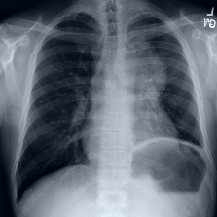
\includegraphics[width=8cm,height=8cm]{xray.png}};




%%%%%%%%%%%%%%%%%%%%%%%%%%%%%%%%%%%%%%%%%%%%%%%%%%%%%%%%%%%%%%%%%%%%%%%%%%%%%%%%%%%%%%%%
%% Draw Encoder
%%%%%%%%%%%%%%%%%%%%%%%%%%%%%%%%%%%%%%%%%%%%%%%%%%%%%%%%%%%%%%%%%%%%%%%%%%%%%%%%%%%%%%%%
% conv1_1,conv1_2



%%%%%%%%%%%%%%%%%%%%%%%%%                           Unet                         %%%%%%%%%%%%%%%%%%%%%%%%%%%%%%%%

\tikzstyle{connection}=[ultra thick,every node/.style={sloped,allow upside down},draw=\edgecolor,opacity=0.7]
\tikzstyle{copyconnection}=[ultra thick,every node/.style={sloped,allow upside down},draw={rgb:blue,4;red,1;green,1;black,3},opacity=0.7]

\pic[shift={(0,14,0)}] at (0,0,0) {Box={name=cr1,%
        font=\Large,caption=Double Conv,zlabel=,fill=\DoubleConv,
        height=40,width={2},depth=40}};

%\pic[shift={(0.75,0,0)}] at (ucr1a-east) {Box={name=out,font=\Large,caption=Softmax,%
%        zlabel=I,fill=\SoftmaxColor,height=40,width=1,depth=40}};


%pool1
\pic[shift={(2.2,0,0)}] at (cr1-east) {Box={name=p1,%
        fill=\PoolColor,opacity=0.5,height=32,width=3,depth=32}};
%%%%%%%%%%
% conv2_1,conv2_2
\pic[shift={(1,0,0)}] at (p1-east) {Box={name=cr2,%
        font=\Large,caption=Down Block 1,zlabel=I/2,fill=\DoubleConv,%bandfill=\ConvReluColor,%
        height=32,width=4,depth=32}};

%pool2
\pic[shift={(2.2,0,0)}] at (cr2-east) {Box={name=p2,%
        fill=\PoolColor,opacity=0.5,height=25,width=4,depth=25}};
%%%%%%%%%%
% conv3_1,conv3_2
\pic[shift={(1,0,0)}] at (p2-east) {Box={name=cr3,%
        font=\Large,caption= Down Block 2,zlabel=,fill=\DoubleConv, %bandfill=\ConvReluColor,%
        height=25,width=4.5,depth=25}};
%pool3
\pic[shift={(2.2,0,0)}] at (cr3-east) {Box={name=p3,%
        fill=\PoolColor,opacity=0.5,height=16,width=6,depth=16}};
%%%%%%%%%%
% conv4_1,conv4_2,conv4_3
\pic[shift={(1,0,0)}] at (p3-east) {Box={name=cr4,%
        font=\Large,caption=Down Block 3,zlabel=,fill=\DoubleConv, %,bandfill=\ConvReluColor,%
        height=16,width=6,depth=16}};
%pool4
\pic[shift={(2.2,0,0)}] at (cr4-east) {Box={name=p4,%
        fill=\PoolColor,opacity=0.5,height=8,width=8,depth=8}};
%%%%%%%%%%%%%%%%%%%%%%%%%%%%%%%%%%%%%%%%%%%%%%%%%%%%%%%%%%%%%%%%%%%%%%%%%%%%%%%%%%%%%%%%
%% Bottleneck
%%%%%%%%%%%%%%%%%%%%%%%%%%%%%%%%%%%%%%%%%%%%%%%%%%%%%%%%%%%%%%%%%%%%%%%%%%%%%%%%%%%%%%%%% conv5_1,conv5_2,conv5_3
\pic[shift={(1,0,0)}] at (p4-east) {Box={name=cr5,font=\Large,caption=Bottleneck Conv,%
        font=\Large,caption= Down Block 4,zlabel=,fill=\DoubleConv,%bandfill=\ConvReluColor,%
        height=8,width=8,depth=8}};
%%%%%%%%%%%%%%%%%%%%%%%%%%%%%%%%%%%%%%%%%%%%%%%%%%%%%%%%%%%%%%%%%%%%%%%%%%%%%%%%%%%%%%%%
%% Draw Decoder 
%%%%%%%%%%%%%%%%%%%%%%%%%%%%%%%%%%%%%%%%%%%%%%%%%%%%%%%%%%%%%%%%%%%%%%%%%%%%%%%%%%%%%%%%
%% unpool4, 
\pic[shift={(2.2,0,0)}] at (cr5-east) {Box={name=up4,%
        fill=\UnpoolColor,opacity=0.6,height=16,width=6,depth=16}};

\pic[shift={(1,0,0)}] at (up4-east) {Box={name=ucr4,%
       font=\Large,caption=Up Block 1,fill=\ConvTransColor,%bandfill=\ConvReluColor,%
        height=16,width=6,depth=16}};

%%%%%%%%%%
%% unpool3, 
\pic[shift={(2.2,0,0)}] at (ucr4-east) {Box={name=up3,%
        fill=\UnpoolColor,opacity=0.6,height=25,width=4.5,depth=25}};
\pic[shift={(1,0,0)}] at (up3-east) {Box={name=ucr3,%
        font=\Large,caption=Up Block 2,fill=\ConvTransColor, %bandfill=\ConvReluColor,%
        height=25,width=4.5,depth=25}};
%%%%%%%%%%
%% unpool2, 
\pic[shift={(2.2,0,0)}] at (ucr3-east) {Box={name=up2,%
        fill=\UnpoolColor,opacity=0.6,height=32,width=3.5,depth=32}};
\pic[shift={(1,0,0)}] at (up2-east) {Box={name=ucr2,%
        font=\Large,caption=Up Block 3,fill=\ConvTransColor, %,bandfill=\ConvReluColor,%
        height=32,width=3.5,depth=32}};
%%%%%%%%%%
%% unpool1, 
\pic[shift={(2.2,0,0)}] at (ucr2-east) {Box={name=up1,%
        fill=\UnpoolColor,opacity=0.6,height=40,width=3,depth=40}};
\pic[shift={(1,0,0)}] at (up1-east) {Box={name=ucr1,%
        font=\Large,caption=Up Block 4,fill=\ConvTransColor, %bandfill=\ConvReluColor,%
        height=40,width=3,depth=40}};
%%%%%%%%%%%%%%%%%%%%%%%%%%%%%%%%%%%%%%%%%%%%%%%%%%%%%%%%%%%%%%%%%%%%%%%%%%%%%%%%%%%%%%%%
%% Classifier 
%%%%%%%%%%%%%%%%%%%%%%%%%%%%%%%%%%%%%%%%%%%%%%%%%%%%%%%%%%%%%%%%%%%%%%%%%%%%%%%%%%%%%%%%%
\pic[shift={(2,0,0)}] at (ucr1-east) {Box={name=out,font=\Large,caption=Softmax,%
        zlabel=I,fill=\SoftmaxColor,height=40,width=1.5,depth=40}};
        
\pic[shift={(-3.6,0,0)}] at (cr1-east) {Box={name=unet,caption=UNet Segmentor, font=\huge,%
        fill=\DenseBlockColor,opacity=0,height=70,width=245,depth=0}};
%%%%%%%%%%%%%%%%%%%%%%%%%%%%%%%%%%%%%%%%%%%%%%%%%%%%%%%%%%%%%%%%%%%%%%%%%%%%%%%%%%%%%%%
% Draw connections
%%%%%%%%%%%%%%%%%%%%%%%%%%%%%%%%%%%%%%%%%%%%%%%%%%%%%%%%%%%%%%%%%%%%%%%%%%%%%%%%%%%%%%%
\draw [connection]  (cr1-east)    -- node {\midarrow} (p1-west);
\draw [connection]  (cr2-east)    -- node {\midarrow} (p2-west);
\draw [connection]  (cr3-east)    -- node {\midarrow} (p3-west);
\draw [connection]  (cr4-east)    -- node {\midarrow} (p4-west);

\draw [connection]  (up4-east)    -- node {\midarrow} (ucr4-west);
\draw [connection]  (up3-east)    -- node {\midarrow} (ucr3-west);
\draw [connection]  (up2-east)    -- node {\midarrow} (ucr2-west);
\draw [connection]  (up1-east)    -- node {\midarrow} (ucr1-west);

\draw [connection]  (p1-east)    -- node {\midarrow} (cr2-west);
\draw [connection]  (p2-east)    -- node {\midarrow} (cr3-west);
\draw [connection]  (p3-east)    -- node {\midarrow} (cr4-west);
\draw [connection]  (p4-east)    -- node {\midarrow} (cr5-west);
\draw [connection]  (cr5-east)   -- node {\midarrow} (up4-west);

\draw [connection]  (ucr4-east) -- node {\midarrow} (up3-west);
\draw [connection]  (ucr3-east) -- node {\midarrow} (up2-west);
\draw [connection]  (ucr2-east) -- node {\midarrow} (up1-west);
\draw [connection]  (ucr1-east) -- node {\midarrow} (out-west);
%\draw [connection]  (out-east)   -- node {\midarrow} ++(2,0,0);
%
\path (cr4-southeast) -- (cr4-northeast) coordinate[pos=1.25] (cr4-top) ;
\path (cr3-southeast) -- (cr3-northeast) coordinate[pos=1.25] (cr3-top) ;
\path (cr2-southeast) -- (cr2-northeast) coordinate[pos=1.25] (cr2-top) ;
\path (cr1-southeast) -- (cr1-northeast) coordinate[pos=1.25] (cr1-top) ;
%

\path (up4-southeast) -- (up4-northeast) coordinate[pos=1.25] (up4-top) ;
\path (up3-southeast) -- (up3-northeast) coordinate[pos=1.25] (up3-top) ;
\path (up2-southeast) -- (up2-northeast) coordinate[pos=1.25] (up2-top) ;
\path (up1-southeast) -- (up1-northeast) coordinate[pos=1.25] (up1-top) ;
%\path (cr3-southeast) -- (cr3-northeast) coordinate[pos=1.25] (cr3-top) ;
%\path (cr2-southeast) -- (cr2-northeast) coordinate[pos=1.25] (cr2-top) ;
%\path (cr1-southeast) -- (cr1-northeast) coordinate[pos=1.25] (cr1-top) ;


%\path (cat4-south)  -- (cat4-north)  coordinate[pos=1.25] (cat4-top) ;
%\path (cat3-south)  -- (cat3-north)  coordinate[pos=1.25] (cat3-top) ;
%\path (cat2-south)  -- (cat2-north)  coordinate[pos=1.25] (cat2-top)  ;
%\path (cat1-south)  -- (cat1-north)  coordinate[pos=1.25] (cat1-top)  ;
%%
\draw [copyconnection]  (cr4-east)  
-- node {\copymidarrow}(cr4-top)
-- node {\copymidarrow}(up4-top)
-- node {\copymidarrow} (up4-east);

\draw [copyconnection]  (cr3-east)  
-- node {\copymidarrow}(cr3-top)
-- node {\copymidarrow}(up3-top)
-- node {\copymidarrow} (up3-east);

\draw [copyconnection]  (cr2-east)  
-- node {\copymidarrow}(cr2-top)
-- node {\copymidarrow}(up2-top)
-- node {\copymidarrow} (up2-east);

\draw [copyconnection]  (cr1-east)  
-- node {\copymidarrow}(cr1-top)
-- node {\copymidarrow}(up1-top)
-- node {\copymidarrow} (up1-east);



%%%%%%%%%%%%%%%%%%%%%%%%%%%%%%%%%%        End of Unet            %%%%%%%%%%%%%%%%%%%%%%%%%%%%%%%%%%%%%%%%%







% conv1_1,conv1_2,%pool1
\pic[shift={(0,0,0)}] at (0,0,0) {Box={name=c1a,font=\Large,caption=conv1,%
        font=\Large,caption=Conv 7x7,zlabel=,fill=\ConvColor,%bandfill=\ConvReluColor,%
        height=40,width=2,depth=40}};

\pic[shift={(0.5,0,0)}] at (c1a-east) {Box={name=p1a,%
        caption=Pool 3x3,fill=\PoolColor,opacity=0.5,height=25,width=2,depth=25}};

\pic[shift={(2,0,0)}] at (p1a-east) {Box={name=block1a,%
        fill=\PoolColor, font=\Large,caption= Dense Block 1, opacity=0.5,height=30,width=40,depth=30,opacity=0.1}};

\pic[shift={(0.8,0,0)}] at (block1a-west) {Box={name=block1a1,%
        fill=\DenseBlockColor,opacity=0.9,height=25,width=2,depth=25}};
\pic[shift={(0.8,0,0)}] at (block1a1-east) {Box={name=block1a2,%
        fill=\DenseBlockColor,opacity=0.8,height=25,width=2,depth=25}};
\pic[shift={(0.8,0,0)}] at (block1a2-east) {Box={name=block1a3,%
        fill=\DenseBlockColor,opacity=0.7,height=25,width=2,depth=25}};
\pic[shift={(0.8,0,0)}] at (block1a3-east) {Box={name=block1a4,%
        fill=\DenseBlockColor,opacity=0.6,height=25,width=2,depth=25}};
\pic[shift={(0.8,0,0)}] at (block1a4-east) {Box={name=block1a5,%
        fill=\DenseBlockColor,opacity=0.5,height=25,width=2,depth=25}};
\pic[shift={(0.8,0,0)}] at (block1a5-east) {Box={name=block1a6,%
        fill=\DenseBlockColor,opacity=0.4,height=25,width=2,depth=25}};

% section 2 

% conv1_1,conv1_2,%pool1
\pic[shift={(1.5,0,0)}] at (block1a6-east) {Box={name=c2a,font=\Large,caption=conv1,%
        font=\Large,caption=Conv 1x1,zlabel=,fill=\ConvColor,%bandfill=\ConvReluColor,%
        height=25,width=2,depth=25}};

\pic[shift={(0.5,0,0)}] at (c2a-east) {Box={name=p2a,%
        caption=Pool 2x2,fill=\PoolColor,opacity=0.5,height=15,width=2.5,depth=15}};

\pic[shift={(1.5,0,0)}] at (p2a-east) {Box={name=block2a,%
        fill=\PoolColor,font=\Large,caption= Dense Block 2,opacity=0.5,height=20,width=38,depth=20,opacity=0.1}};

\pic[shift={(0.8,0,0)}] at (block2a-west) {Box={name=block2a1,%
        fill=\DenseBlockColor,opacity=0.9,height=15,width=2.5,depth=15}};
\pic[shift={(0.8,0,0)}] at (block2a1-east) {Box={name=block2a2,%
        fill=\DenseBlockColor,opacity=0.8,height=15,width=2.5,depth=15}};
\pic[shift={(0.8,0,0)}] at (block2a2-east) {Box={name=block2a3,%
        fill=\DenseBlockColor,opacity=0.7,height=15,width=2.5,depth=15}};
\pic[shift={(2.6,0,0)}] at (block2a3-east) {Box={name=block2a4,%
        fill=\DenseBlockColor,opacity=0.6,height=15,width=2.5,depth=15}};
%\pic[shift={(0.8,0,0)}] at (block2a4-east) {Box={name=block2a5,%
%        fill=\DenseBlockColor,opacity=0.5,height=15,width=2,depth=15}};
%\pic[shift={(0.8,0,0)}] at (block2a5-east) {Box={name=block2a6,%
%        fill=\DenseBlockColor,opacity=0.4,height=15,width=2,depth=15}};


% section 3 
% conv1_1,conv1_2,%pool1
\pic[shift={(1.5,0,0)}] at (block2a4-east) {Box={name=c3a,font=\Large,caption=conv1,%
        font=\Large,caption=Conv 1x1,zlabel=,fill=\ConvColor,%bandfill=\ConvReluColor,%
        height=15,width=2.5,depth=15}};

\pic[shift={(0.5,0,0)}] at (c3a-east) {Box={name=p3a,%
        caption=Pool 2x2,fill=\PoolColor,opacity=0.5,height=10,width=2.5,depth=10}};

\pic[shift={(1.1,0,0)}] at (p3a-east) {Box={name=block3a,%
        fill=\PoolColor,font=\Large,caption= Dense Block 3,opacity=0.5,height=14,width=38,depth=14,opacity=0.1}};

\pic[shift={(0.6,0,0)}] at (block3a-west) {Box={name=block3a1,%
        fill=\DenseBlockColor,opacity=0.9,height=10,width=3,depth=10}};
\pic[shift={(0.8,0,0)}] at (block3a1-east) {Box={name=block3a2,%
        fill=\DenseBlockColor,opacity=0.8,height=10,width=3,depth=10}};
\pic[shift={(0.8,0,0)}] at (block3a2-east) {Box={name=block3a3,%
        fill=\DenseBlockColor,opacity=0.7,height=10,width=3,depth=10}};
\pic[shift={(2.6,0,0)}] at (block3a3-east) {Box={name=block3a4,%
        fill=\DenseBlockColor,opacity=0.6,height=10,width=3,depth=10}};


% Section 4 
% conv1_1,conv1_2,%pool1
\pic[shift={(1,0,0)}] at (block3a4-east) {Box={name=c4a,font=\Large,caption=conv1,%
        font=\Large,caption=Conv 1x1,zlabel=,fill=\ConvColor,%bandfill=\ConvReluColor,%
        height=10,width=3.5,depth=10}};

\pic[shift={(0.5,0,0)}] at (c4a-east) {Box={name=p4a,%
        caption=Pool 2x2, fill=\PoolColor,opacity=0.5,height=7,width=3.5,depth=7}};

\pic[shift={(0.8,0,0)}] at (p4a-east) {Box={name=block4a,%
        fill=\PoolColor,font=\Large,caption= Dense Block 4,opacity=0.5,height=9,width=38,depth=9,opacity=0.1}};

\pic[shift={(0.4,0,0)}] at (block4a-west) {Box={name=block4a1,%
        fill=\DenseBlockColor,opacity=0.9,height=7,width=3.5,depth=7}};
\pic[shift={(0.8,0,0)}] at (block4a1-east) {Box={name=block4a2,%
        fill=\DenseBlockColor,opacity=0.8,height=7,width=3.5,depth=7}};
\pic[shift={(0.8,0,0)}] at (block4a2-east) {Box={name=block4a3,%
        fill=\DenseBlockColor,opacity=0.7,height=7,width=3.5,depth=7}};
\pic[shift={(2.6,0,0)}] at (block4a3-east) {Box={name=block4a4,%
        fill=\DenseBlockColor,opacity=0.6,height=7,width=3.5,depth=7}};
 \node[text width=20cm, align=center,font=\Large\sffamily, shift={(1.9,-0.5,0)}] at (block4a4-east) {(HxWxC)};
\pic[shift={(-3.6,-0.8,0)}] at (c1a-east) {Box={name=densenet,caption=Densenet Feature Extractor, font=\huge,%
        fill=\DenseBlockColor,opacity=0,height=65,width=245,depth=0}};
        
        

%%% arc connections  
%%%%%%%%%%%%% all the center connections %%%%%%%%%%%%%%%%
\draw [connection]  (c1a-east) -- node {\midarrow} (p1a-west);
\draw [connection]  (c2a-east) -- node {\midarrow} (p2a-west);
\draw [connection]  (c3a-east) -- node {\midarrow} (p3a-west);
\draw [connection]  (c4a-east) -- node {\midarrow} (p4a-west);

\draw [connection]  (p1a-east) -- node {\midarrow} (block1a1-west);
\draw [connection]  (p2a-east) -- node {\midarrow} (block2a1-west);
\draw [connection]  (p3a-east) -- node {\midarrow} (block3a1-west);
\draw [connection]  (p4a-east) -- node {\midarrow} (block4a1-west);

%\draw [connection]  (p1a-east) -- node {\midarrow} (block1a1-west);
\draw [connection]  (block1a6-east) -- node {\midarrow} (c2a-west);
\draw [connection]  (block2a4-east) -- node {\midarrow} (c3a-west);
\draw [connection]  (block3a4-east) -- node {\midarrow} (c4a-west);


\draw [connection]  (block1a1-east) -- node {\midarrow} (block1a2-west);
\draw [connection]  (block1a2-east) -- node {\midarrow} (block1a3-west);
\draw [connection]  (block1a3-east) -- node {\midarrow} (block1a4-west);
\draw [connection]  (block1a4-east) -- node {\midarrow} (block1a5-west);
\draw [connection]  (block1a5-east) -- node {\midarrow} (block1a6-west);


\draw [connection]  (block2a1-east) -- node {\midarrow} (block2a2-west);
\draw [connection]  (block2a2-east) -- node {\midarrow} (block2a3-west);
%\draw [connection]  (block2a3-east) -- node {\midarrow} (block2a4-west);

\draw [connection]  (block3a1-east) -- node {\midarrow} (block3a2-west);
\draw [connection]  (block3a2-east) -- node {\midarrow} (block3a3-west);
%\draw [connection]  (block3a3-east) -- node {\midarrow} (block3a4-west);


\draw [connection]  (block4a1-east) -- node {\midarrow} (block4a2-west);
\draw [connection]  (block4a2-east) -- node {\midarrow} (block4a3-west);
%\draw [connection]  (block4a3-east) -- node {\midarrow} (block4a4-west);





%%%%% dense conection for block1 %%%%%%%%%%%%%%% 
\draw [- > ] (block1a1-north) to [bend left=90] (block1a2-north);

\draw [- > ] (block1a1-north) to [bend left=90] (block1a3-north);
\draw [- > ] (block1a2-north) to [bend left=90] (block1a3-north);

\draw [- > ] (block1a1-north) to [bend left=90] (block1a4-north);
\draw [- > ] (block1a2-north) to [bend left=90] (block1a4-north);
\draw [- > ] (block1a3-north) to [bend left=90] (block1a4-north);

\draw [- > ] (block1a1-north) to [bend left=90] (block1a5-north);
\draw [- > ] (block1a2-north) to [bend left=90] (block1a5-north);
\draw [- > ] (block1a3-north) to [bend left=90] (block1a5-north);
\draw [- > ] (block1a4-north) to [bend left=90] (block1a5-north);

\draw [- > ] (block1a1-north) to [bend left=90] (block1a6-north);
\draw [- > ] (block1a2-north) to [bend left=90] (block1a6-north);
\draw [- > ] (block1a3-north) to [bend left=90] (block1a6-north);
\draw [- > ] (block1a4-north) to [bend left=90] (block1a6-north);
\draw [- > ] (block1a5-north) to [bend left=90] (block1a6-north);



%%%%% dense conection for block2 %%%%%%%%%%%%%%% 
\draw [- > ] (block2a1-north) to [bend left=90] (block2a2-north);

\draw [- > ] (block2a1-north) to [bend left=90] (block2a3-north);
\draw [- > ] (block2a2-north) to [bend left=90] (block2a3-north);

\draw [- > ] (block2a1-north) to [bend left=90] (block2a4-north);
\draw [- > ] (block2a2-north) to [bend left=90] (block2a4-north);
\draw [- > ] (block2a3-north) to [bend left=90] (block2a4-north);

% for the dots 
\node at ($(block2a3-northwest)!.65!(block2a4-northwest)$) {\ldots};
\node at ($(block2a3-west)!.65!(block2a4-west)$) {\ldots};
\node at ($(block2a3-southwest)!.65!(block2a4-southwest)$) {\ldots};

%%%%%%%%% dense conection for block3 %%%%%%%%%%%
\draw [- > ] (block3a1-north) to [bend left=90] (block3a2-north);

\draw [- > ] (block3a1-north) to [bend left=90] (block3a3-north);
\draw [- > ] (block3a2-north) to [bend left=90] (block3a3-north);

\draw [- > ] (block3a1-north) to [bend left=90] (block3a4-north);
\draw [- > ] (block3a2-north) to [bend left=90] (block3a4-north);
\draw [- > ] (block3a3-north) to [bend left=90] (block3a4-north);

% for the dots 
\node at ($(block3a3-northwest)!.65!(block3a4-northwest)$) {\ldots};
\node at ($(block3a3-west)!.65!(block3a4-west)$) {\ldots};
\node at ($(block3a3-southwest)!.65!(block3a4-southwest)$) {\ldots};


%%%%%%%%% dense conection for block4 %%%%%%%%%%%%%%% 
\draw [- > ] (block4a1-north) to [bend left=90] (block4a2-north);

\draw [- > ] (block4a1-north) to [bend left=90] (block4a3-north);
\draw [- > ] (block4a2-north) to [bend left=90] (block4a3-north);

\draw [- > ] (block4a1-north) to [bend left=90] (block4a4-north);
\draw [- > ] (block4a2-north) to [bend left=90] (block4a4-north);
\draw [- > ] (block4a3-north) to [bend left=90] (block4a4-north);

% for the dots 
\node at ($(block4a3-northwest)!.65!(block4a4-northwest)$) {\ldots};
\node at ($(block4a3-west)!.65!(block4a4-west)$) {\ldots};
\node at ($(block4a3-southwest)!.65!(block4a4-southwest)$) {\ldots};
%\draw (block4a3-north) -- (block4a4-north);

%%%%%%%%%%%%%%%%%%%%%%%%%%%%%%                              %%%%%%%%%%%%%%%%%%%%%%%%%%%%%%%%%%%
%%%%%%%%%%%%%%%%%%%%%%%%%%%%         Attention module     %%%%%%%%%%%%%%%%%%%%%%%%%%%%%%%%%%%%
%%%%%%%%%%%%%%%%%%%%%%%%%%%%%%%                          %%%%%%%%%%%%%%%%%%%%%%%%%%%%%%%%%%%%

\pic[shift={(5,0,0)}] at (out-east) {Box={name=ppb,font=\Large,caption=Post Processing Block,%
        fill={rgb:yellow,2;green,2;blue,7},height=25,width=15,depth=25}};
\node[canvas is zy plane at x=55] (lungmask) at (0,14,0) {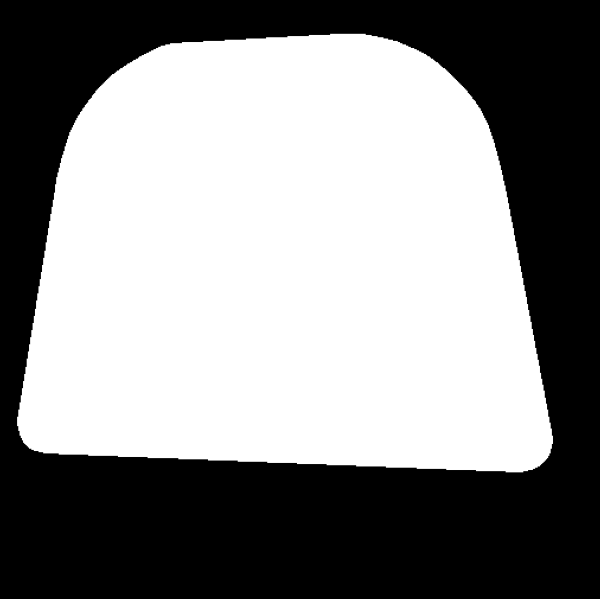
\includegraphics[width=5cm,height=5cm]{lungmask.png}};
\pic[shift={(8,0,0)}] at (ppb-east) {Box={name=slab,font=\Large,caption=Segmentation Lung Attention Block,%
        fill={rgb:gray,5;black,5},height=18,width=18,depth=18}};
        
 \node[text width=20cm, align=center,font=\Large\sffamily, shift={(1.2,-3.5,0)}] at (slab-south) {(HxWxC)};


\node[canvas is zy plane at x=55] (pic1) at (-5,3,0) {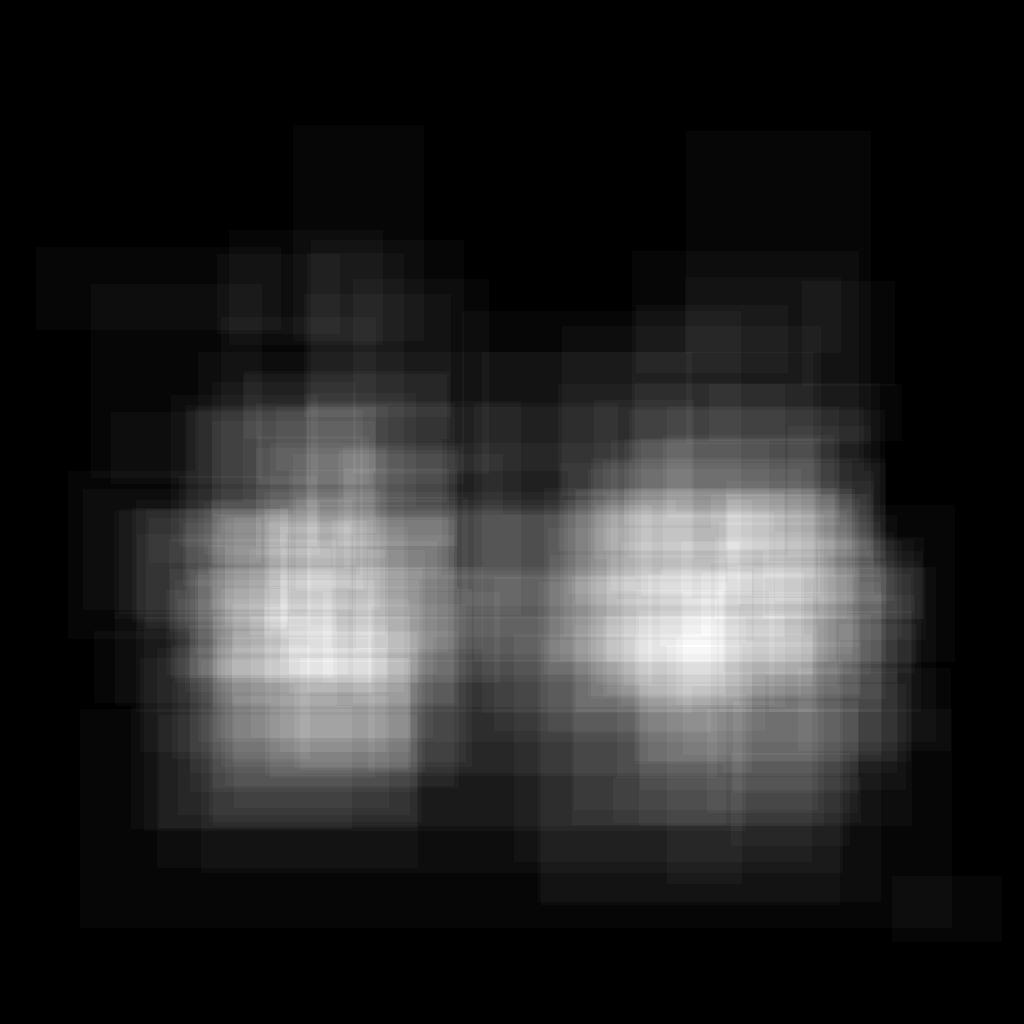
\includegraphics[width=5cm,height=5cm]{mask_0.jpg}};
\pic[shift={(3,0,0)}] at (pic1) {Box={name=attn1a,font=\Large,caption=Disease 1 Attention Block,%
        fill={rgb:gray,5;black,5},height=18,width=18,depth=18}};
 \node[text width=20cm, align=center,font=\Large\sffamily, shift={(1.9,-0.5,0)}] at (attn1a-east) {(HxWxC)};
\pic[shift={(3.5,0,0)}] at (attn1a-east) {Ball={name=cat1,fill=\ConcatColor,radius=2.5,logo=$C$}};
\pic[shift={(7,0,0)}] at (attn1a-east) {Box={name=attn2a,font=\Large,caption=GAP,%
        fill=\PoolColor,height=12,width=3,depth=12}};
\pic[shift={(1.5,0,0)}] at (attn2a-east) {Box={name=attn3a,font=\Large,caption=Classifier1 Conv 1x1,%
        fill=\ConvColor,height=12,width=3,depth=12}};
\pic[shift={(3,5,0)}] at (attn3a-east) {Box={name=scorea,font=\Large,caption=Disease 1 Probability Score,%
        fill=\SoftmaxColor,height=5,width=10,depth=0}};
%\pic[shift={(3,-2,0)}] at (attn3a-east) {Box={name=heatmapa,font=\Large,caption=1st Heatmap,%
%        fill={rgb:magenta,5},opacity=0.2, height=18,width=18,depth=0}};
\node[canvas is zy plane at x=75] (heatmap1) at (-4.5,2.5,0) {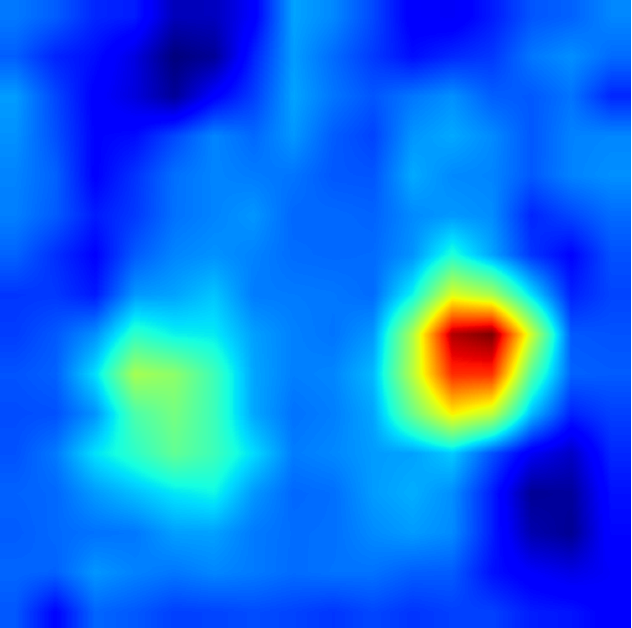
\includegraphics[width=5cm,height=5cm]{heatmapc.png}};
\node[text width=20cm, align=center,font=\Large\sffamily, shift={(0,-3.8,0)}] at (heatmap1) {Disease 1 Heatamp (HxW)};

\node[canvas is zy plane at x=55] (pic2) at (-5,-6,0) {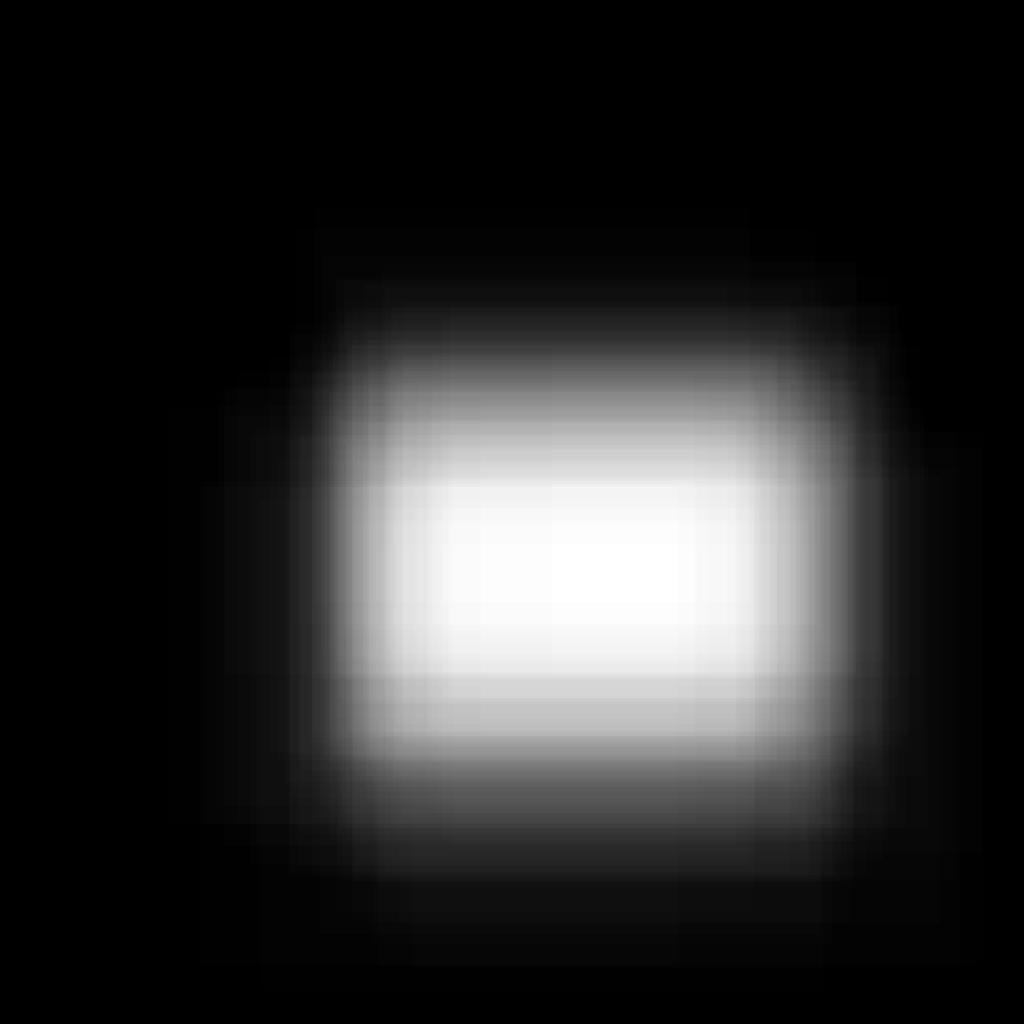
\includegraphics[width=5cm,height=5cm]{mask_1.jpg}};
\pic[shift={(3,0,0)}] at (pic2) {Box={name=attn1b,font=\Large,caption=Disease 2 Attention Block,%
        fill={rgb:gray,5;black,5},height=18,width=18,depth=18}};
 \node[text width=20cm, align=center,font=\Large\sffamily, shift={(1.9,-0.5,0)}] at (attn1b-east) {(HxWxC)};
\pic[shift={(3.5,0,0)}] at (attn1b-east) {Ball={name=cat2,fill=\ConcatColor,radius=2.5,logo=$C$}};
\pic[shift={(7,0,0)}] at (attn1b-east) {Box={name=attn2b,font=\Large,caption=GAP,%
        fill=\PoolColor,height=12,width=3,depth=12}};
\pic[shift={(1.5,0,0)}] at (attn2b-east) {Box={name=attn3b,font=\Large,caption=Classifier2 Conv 1x1,%
        fill=\ConvColor,height=12,width=3,depth=12}};
\pic[shift={(3,4,0)}] at (attn3b-east) {Box={name=scoreb,font=\Large,caption=Disease 2 Probability Score,%
        fill=\SoftmaxColor,height=5,width=10,depth=0}};
%\pic[shift={(3,-2,0)}] at (attn3b-east) {Box={name=heatmapb,font=\Large,caption=2nd Heatmap,%
%        fill={rgb:magenta,5},opacity=0.2, height=18,width=18,depth=0}};
\node[canvas is zy plane at x=75] (heatmap2) at (-4.5,-7.5,0) {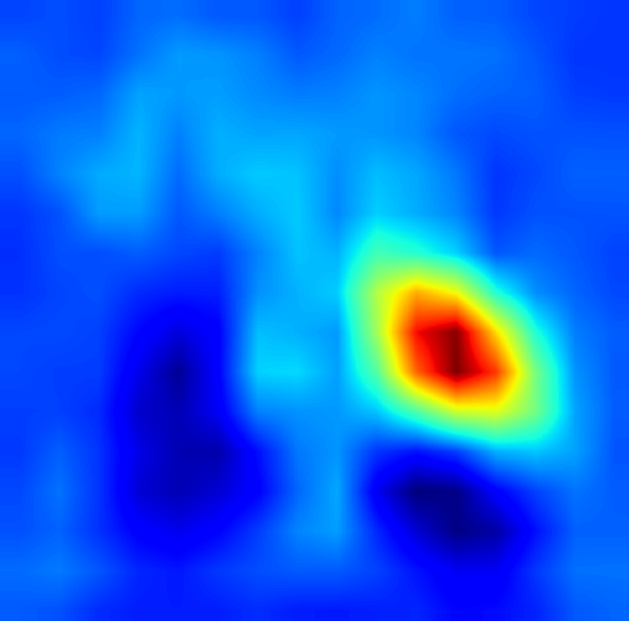
\includegraphics[width=5cm,height=5cm]{heatmapb.png}};
\node[text width=20cm, align=center,font=\Large\sffamily, shift={(0,-3.8,0)}] at (heatmap2) {Disease 2 Heatamp (HxW)};

\node[canvas is zy plane at x=55] (pic3) at (-5,-18,0) {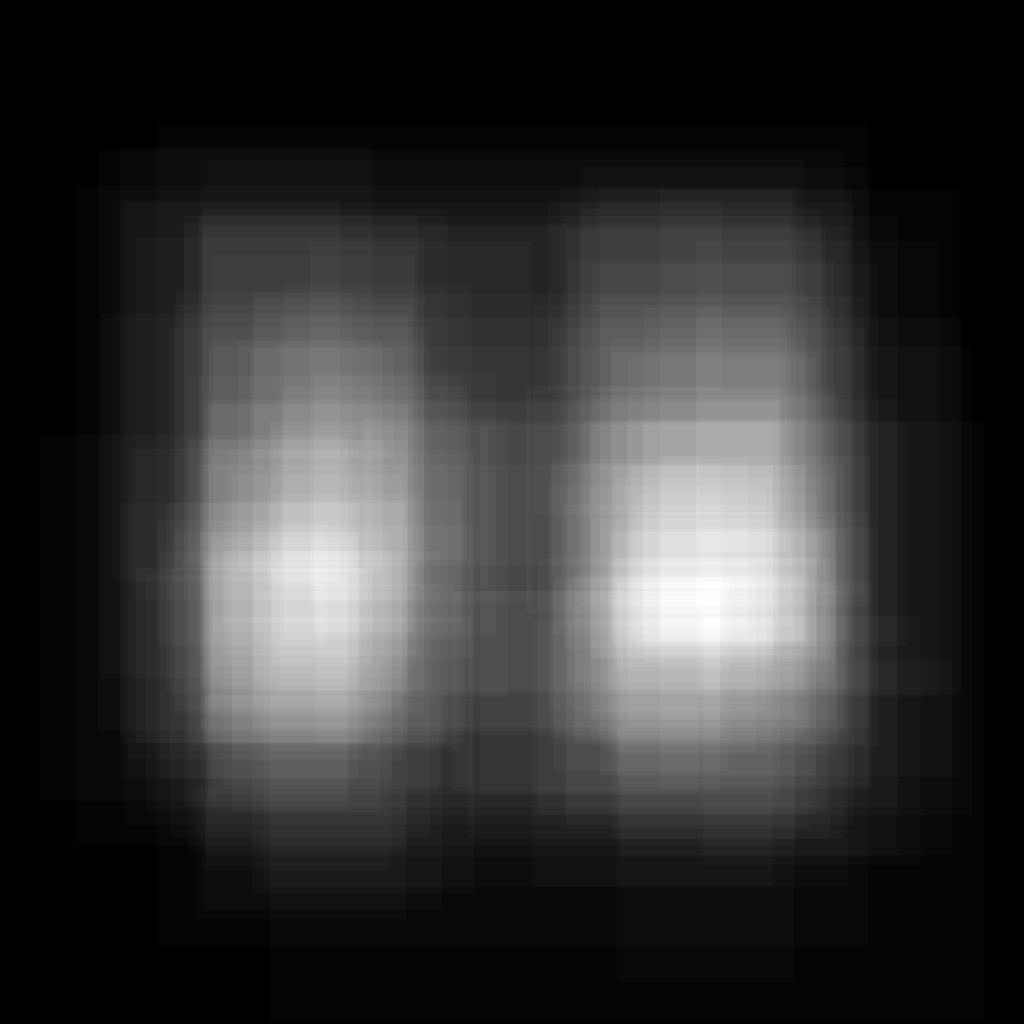
\includegraphics[width=5cm,height=5cm]{mask_6.jpg}};
\pic[shift={(3,0,0)}] at (pic3) {Box={name=attn1c,font=\Large,caption=Disease N Attention Block,%
        fill={rgb:gray,5;black,5},height=18,width=18,depth=18}};
 \node[text width=20cm, align=center,font=\Large\sffamily, shift={(1.9,-0.5,0)}] at (attn1c-east) {(HxWxC)};
\pic[shift={(3.5,0,0)}] at (attn1c-east) {Ball={name=cat3,fill=\ConcatColor,radius=2.5,logo=$C$}};
\pic[shift={(7,0,0)}] at (attn1c-east) {Box={name=attn2c,font=\Large,caption=GAP,%
        fill=\PoolColor,height=12,width=3,depth=12}};
\pic[shift={(1.5,0,0)}] at (attn2c-east) {Box={name=attn3c,font=\Large,caption=ClassifierN Conv 1x1,%
        fill=\ConvColor,height=12,width=3,depth=12}};
\pic[shift={(3,4,0)}] at (attn3c-east) {Box={name=scorec,font=\Large,caption=Disease N Probability Score,%
        fill=\SoftmaxColor,height=5,width=10,depth=0}};
\node[canvas is zy plane at x=75] (heatmap3) at (-4.5,-19.5,0) {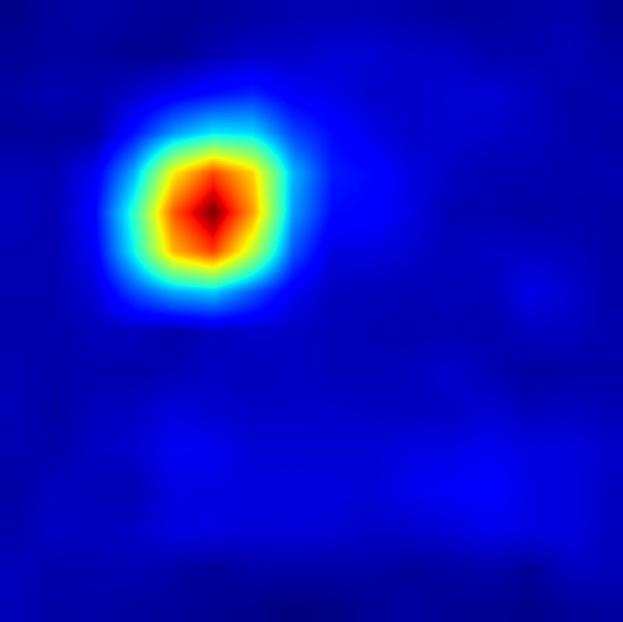
\includegraphics[width=5cm,height=5cm]{heatmapa.png}};
\node[text width=20cm, align=center,font=\Large\sffamily, shift={(0,-3.8,0)}] at (heatmap3) {Disease N Heatamp (HxW)};
        
%\pic[shift={(3,-2,0)}] at (attn3c-east) {Box={name=heatmapc,font=\Large,caption=Nth Heatmap,%
%        fill={rgb:magenta,5},opacity=0.2, height=18,width=18,depth=0}};


%%% adition nodes %%%%%%%
%\pic[shift={(0,10,0)}] at (ucr1-anch) {Ball={name=cat1,fill=\ConcatColor,radius=2.5,logo=$||$}};

%%%%%%%%%%connections%%%%%%%%%%%%%%%%

\draw [connection]  (out-east) -- node {\midarrow} (ppb-west);
\draw [connection]  (ppb-east) -- node {\midarrow} ++(2.5, 0,0); %)%(slab-west);
\draw [connection]  (lungmask) -- node {\midarrow} (slab-west);

\draw [connection]  (pic1) -- node {\midarrow} (attn1a-west);
\draw [connection]  (attn1a-east) -- node {\midarrow} (cat1-west);
\draw [connection]  (cat1-east) -- node {\midarrow} (attn2a-west);
%\draw [connection]  (attn1b-east) -- node {\midarrow} (attn2b-west);
\draw [connection]  (attn2a-east) -- node {\midarrow} (attn3a-west);
%\draw [connection]  (attn3a-east) -- node {\midarrow} (scorea-west);
%\draw [connection] (attn3a-east) to [bend left=30,color={rgb:red,5}]node {\midarrow} (scorea-west);
\draw [connection] (attn3a-east) to [bend left=30]node {\midarrow} (scorea-west);
\draw [connectionred] (cat1-east) to [bend left=-30](attn3a-west);
\draw [connectionred] (attn3a-east) to [bend left=-30]node {\midarrow} (heatmap1);



\draw [connection]  (pic2) -- node {\midarrow} (attn1b-west);
\draw [connection]  (attn1b-east) -- node {\midarrow} (cat2-west);
\draw [connection]  (cat2-east) -- node {\midarrow} (attn2b-west);
\draw [connection]  (attn2b-east) -- node {\midarrow} (attn3b-west);
%\draw [connection]  (attn3b-east) -- node {\midarrow} (scoreb-west);
\draw [connection] (attn3b-east) to [bend left=30]node {\midarrow} (scoreb-west);
\draw [connectionred] (cat2-east) to [bend left=-30](attn3b-west);
\draw [connectionred] (attn3b-east) to [bend left=-30]node {\midarrow} (heatmap2);


\draw [connection]  (pic3) -- node {\midarrow} (attn1c-west);
\draw [connection]  (attn1c-east) -- node {\midarrow} (cat3-west);
\draw [connection]  (cat3-east) -- node {\midarrow} (attn2c-west);
%\draw [connection]  (attn1c-east) -- node {\midarrow} (attn2c-west);
\draw [connection]  (attn2c-east) -- node {\midarrow} (attn3c-west);
%\draw [connection]  (attn3c-east) -- node {\midarrow} (scorec-west);
\draw [connection] (attn3c-east) to [bend left=30]node {\midarrow} (scorec-west);
\draw [connectionred] (cat3-east) to [bend left=-30] (attn3c-west);
\draw [connectionred] (attn3c-east) to [bend left=-30]node {\midarrow} (heatmap3);


\draw(slab-south)[->,line width =0.5mm,color=\edgecolor]--++(0,-28,0)--(cat3-north);
\draw(slab-south)[->,line width =0.5mm,color=\edgecolor]--++(0,-16,0)--(cat2-north);
\draw(slab-south)[->,line width =0.5mm,color=\edgecolor]--++(0,-6.5,0)--(cat1-north);
%\draw(slab-south)++(0,-30,0)[color={rgb:green,5;black,5}]--++(0,-30,0);
%\draw(slab-south)[color={rgb:green,5;black,5}]--(cat3-east)++(0,-30,0);

\draw(block4a4-east)[->,line width =0.5mm,color=\edgecolor]--++(3,0,0)--++(0,1.2,0)--(attn1a-southwest);
\draw(block4a4-east)[->,line width =0.5mm,color=\edgecolor]--++(3,0,0)--++(0,-7.8,0)--(attn1b-southwest);
\draw(block4a4-east)[->,line width =0.5mm,color=\edgecolor]--++(3,0,0)--++(0,-19.8,0)--(attn1c-southwest);
\draw(block4a4-east)[->,line width =0.5mm,color=\edgecolor]--++(3,0,0)--++(0,7.8,0)--++(9,0,0)--++(0,4.4,0)--(slab-southwest);

\draw(temp)[->,line width =0.5mm,color=\edgecolor]--++(3,0,0)--++(0,8,0)--(cr1-west);
\draw(temp)[->,line width =0.5mm,color=\edgecolor]--++(3,0,0)--++(0,-6,0)--(c1a-west);


%%%% for the dots in the attention blocks %%%% 
%\path (up4-southeast) -- (up4-northeast) coordinate[pos=1.25] (dot-top1) ;
%\path (up3-southeast) -- (up3-northeast) coordinate[pos=1.25] (dot-top) ;
%\path (up2-southeast) -- (up2-northeast) coordinate[pos=1.25] (up2-top) ;
%\path (up1-southeast) -- (up1-northeast) coordinate[pos=1.25] (up1-top) ;

\node at ($(attn1b-south)+(1,1,0)!.65!(attn2b-south)$) {\ldots};
%\draw (attn1b-south) [line width=0.5mm, color=\edgecolor, dotted] -- (attn2b-south);
\draw (attn1b-south)++(5,-2,0) -- ++(1,0,0) [line width=0.5mm, color=\edgecolor, loosely dotted];
\draw (attn1b-south)++(5,-4,0) -- ++(1,0,0) [line width=0.5mm, color=\edgecolor, loosely dotted];
\draw (attn1b-south)++(5,-6,0) -- ++(1,0,0) [line width=0.5mm, color=\edgecolor, loosely dotted];

\draw (attn1b-south)++(14,-2,0) -- ++(1,0,0) [line width=0.5mm, color=\edgecolor, loosely dotted];
\draw (attn1b-south)++(14,-4,0) -- ++(1,0,0) [line width=0.5mm, color=\edgecolor, loosely dotted];
\draw (attn1b-south)++(14,-6,0) -- ++(1,0,0) [line width=0.5mm, color=\edgecolor, loosely dotted];

\draw (attn1b-south)++(-2,-2,0) -- ++(1,0,0) [line width=0.5mm, color=\edgecolor, loosely dotted];
\draw (attn1b-south)++(-2,-4,0) -- ++(1,0,0) [line width=0.5mm, color=\edgecolor, loosely dotted];
\draw (attn1b-south)++(-2,-6,0) -- ++(1,0,0) [line width=0.5mm, color=\edgecolor, loosely dotted];



%\draw (block4a4-east) [->, line width=0.5mm, color=\edgecolor, dotted] -- ++(3,0,0) -- ++(0,1.2,0) -- (attn1a-southwest);

%\node at ($(attn1b-south)!.65!(attn2b-south)$) {\ldots};
%\node at ($(attn1b-south)!.65!(attn2b-south)$) {\ldots};



%%%%%%%%%%%%%%%%%%%%%%%%%%%%%%%%%%%%%%%%%%%%%%%%%%%%%%%%%%%%%%%%%%%%%%%%%%%%%%%%%%%%%%%%

\end{tikzpicture}
\end{document}\grid
